% ------------------------------------------------------------
% LaTeX Template für die DHBW zum Schnellstart!
% Original: https://github.wdf.sap.corp/vtgermany/LaTeX-Template-DHBW
% ------------------------------------------------------------
% ---- Präambel mit Angaben zum Dokument
\input{Inhalt/00_Latex/praeambel}

% ---- Elektronische Version oder Gedruckte Version?
% ---- Unterschied: Die elektronische Version enthält keinen Platzhalter für die Unterschrift
\usepackage{ifthen}
\newboolean{e-Abgabe}
\setboolean{e-Abgabe}{false}    % false=gedruckte Fassung

% ---- Persönlichen Daten:
\newcommand{\titel}{Emissionszertifikate als umweltpolitisches Instrument gegen den Klimawandel: Theorie und Praxis}
\newcommand{\titelheader}{Emissionszertifikate}
\newcommand{\arbeit}{Seminararbeit VWL 2}
\newcommand{\studiengang}{Wirtschaftsinformatik Software Engineering}
\newcommand{\studienjahr}{2022}
\newcommand{\autor}{Alexander Meinecke}
\newcommand{\autorReverse}{Meinecke, Alexander}
\newcommand{\verfassungsort}{Mannheim}
\newcommand{\matrikelnr}{1522347}
\newcommand{\kurs}{WWI22SEB}
\newcommand{\bearbeitungsmonat}{Dezember 2023}
\newcommand{\abgabe}{25. Januar 2024}
\newcommand{\bearbeitungszeitraum}{Dezember 2023 - 25. Januar 2024}
\newcommand{\firmaName}{SAP SE}
\newcommand{\firmaStrasse}{Dietmar-Hopp-Allee 16}
\newcommand{\firmaPlz}{69190 Walldorf, Deutschland}
\newcommand{\betreuerDhbw}{Prof. Dr. Frank Hubert}

\input{Inhalt/00_Latex/kopfundFusszeile}

% ---- Hilfreiches
\newcommand{\zB}{z.\,B. }   % "z.B." mit kleinem Leeraum dazwischen (ohne wäre nicht korrekt)
\newcommand{\dash}{d.\,h. }

\newcommand{\code}[1]{\texttt{#1}} % Ist einfacher zu schreiben als ständig \texttt und erlaubt
                                   % Änderungen im Nachhinein, wenn man z.B. Inline-Code anders stylen möchte.

% ---- Silbentrennung (falls LaTeX defaults falsch / nicht gewünscht sind)
\hyphenation{HANA}         % anstatt HA-NA
\hyphenation{Graph-Script} % anstatt GraphS-cript

% ---- Beginn des Dokuments
\begin{document}
\setlength{\parindent}{0pt}              % Keine Paragraphen Einrückung.
                                         % Dafür haben wir den Abstand zwischen den Paragraphen.
\setcounter{secnumdepth}{2}              % Nummerierungstiefe fürs Inhaltsverzeichnis
\setcounter{tocdepth}{1}                 % Tiefe des Inhaltsverzeichnisses. Ggf. so anpassen,
                                         % dass das Verzeichnis auf eine Seite passt.
\sffamily                                % Serifenlose Schrift verwenden.

% ---- Vorspann
% ------ Titelseite
\singlespacing
\include{Inhalt/01_Standard/titelseite}  % Titelseite
\newcounter{savepage}
\pagenumbering{Roman}                    % Römische Seitenzahlen
\onehalfspacing

% ------ Erklärung, Sperrvermerk, Abstact
\include{Inhalt/01_Standard/erklaerung}
%\include{Inhalt/01_Standard/sperrvermerk}
%\include{Inhalt/02_Abstract/abstract-en}
%\include{Inhalt/02_Abstract/abstract-de}

% ------ Inhaltsverzeichnis
\singlespacing
\tableofcontents

% ------ Verzeichnisse
\renewcommand*{\chapterpagestyle}{plain}
\pagestyle{plain}
%\include{Inhalt/03_Verzeichnisse/formelgroessen}
\listoffigures % Erzeugen des Abbildungsverzeichnisses 
\chapter*{Abkürzungsverzeichnis}
\addcontentsline{toc}{chapter}{Abkürzungsverzeichnis} % Hinzufügen zum Inhaltsverzeichnis 

\begin{acronym}[WYSISWG] % längstes Kürzel wird verw. für den Abstand zw. Kürzel u. Text

	% Alphabetisch selbst sortieren - nicht verwendete Kürzel rausnehmen!
	\acro{BEHG}{Brennstoffemissionshandelsgesetz}
	\acro{CBAM}{Carbon Border Adjustment Mechanism (dt. Grenzausgleichsmechanismus)}
	\acro{DEHSt}{Deutsche Emissionshandelsstelle}
	\acro{ETS}{Emission Trading System (dt. Emissionshandelssystem)}
	\acro{ICAP}{International Carbon Action Partnership (dt. Internationale Partnerschaft für Emissionshandel)}
	\acro{MSR}{Market Stability Reserve (dt. Marktstabilitätsreserve)}
	\acro{nEHS}{Nationales Emissionshandelssystem}
	\acro{TNAC}{Total Number of Allowances in Circulation (dt. Anzahl der Zertifikate im Umlauf)}

\end{acronym}           
%\listoftables                           % Erzeugen des Tabellenverzeichnisses
%\renewcommand{\lstlistlistingname}{Quellcodeverzeichnis}
%\lstlistoflistings                      % Erzeugen des Listenverzeichnisses
\setcounter{savepage}{\value{page}}


% ---- Inhalt der Arbeit
\cleardoublepage
\pagenumbering{arabic}                  % Arabische Seitenzahlen für den Hauptteil
\setlength{\parskip}{0.5\baselineskip}  % Abstand zwischen Absätzen
\rmfamily
\renewcommand*{\chapterpagestyle}{scrheadings}
\pagestyle{scrheadings}
\onehalfspacing
\chapter{Einleitung}

Der Klimawandel, seine Folgen und den damit verbundenen Handlungsbedarf diesen aufzuhalten sind  

\chapter{Theorie}

Ein Emissionshandelssystem setzt auf das Verursacherprinzip (vgl. \cite[S. 161]{hubert.2020}).
Das bedeutet, dass die Akteure, die tatsächlich für die Emissionen verantwortlich sind, in einer Volkswirtschaft monetär zur Verantwortung gezogen werden.
In einem Emissionshandelssystem werden die Rechte, Treibhausgase zu emittieren, als Zertifikate dargestellt (vgl. \cite[S. 27]{rabe.2018}).
Ein Zertifikat berechtigt den Besitzer, eine Tonne $CO_2$-Äquivalente ($CO_2$e) zu emittieren.
Es wird von Äquivalenten gesprochen, da es neben $CO_2$ verschiedene Treibhausgase gibt, die unterschiedlich stark zum Klimawandel beitragen. $CO_2$ wird als Referenzgröße verwendet.
Es wird hier auch vom 'Global Warming Potential' gesprochen. So hat bspw. Methan ein 28-fach höheres 'Global Warming Potential' als $CO_2$ (vgl. \cite{ub.2023}).
Stößt ein Verursacher mehr $CO_2$e aus, als er Zertifikate besitzt, muss dieser hohe Sanktionszahlungen leisten, die in keinem Verhältnis zu den tatsächlichen 'Ersparnissen' durch den Nichtkauf der Zertifikate stehen und daher ökonomisch keinen Sinn machen (vgl. \cite[S. 181]{hubert.2020}).

Das Kernkonzept eines Emissionshandelssystems ist das sog. 'Cap and Trade' (dt. 'Verknappen und Handeln') (vgl. \cite[S. 134]{rabe.2018}).
Aus den Klimaschutzzielen einer Regierung wird eine Obergrenze (CAP) für die Emissionenzertifikate bis zu einem bestimmten Zeitpunkt festgelegt, also der Zeitpunkt, bis zu dem die Volkswirtschaft klimaneutral sein soll (vgl. \cite[S. 181]{hubert.2020}).
Die Zertifikate unterhalb dieser Obergrenze werden nun jährlich entweder unter Orientierung an dem bisherigen Treibhausgasaustoß eines Verursachers kostenlos oder kostenpflichtig verteilt oder alternativ versteigert (vgl. \cite[S. 181]{hubert.2020}).

Aus dem bislang öffentlichen Gut 'Emissionen ausstoßen' wird so durch die Unterteilung in kostenpflichtige Zertifikate zu einem knappen Gut, mit dem nach der Ausgabe marktwirtschaftlich gewirtschaftet werden kann (Trade) (vgl. \cite[S. 17]{hubert.2020}).
Die Angebotsobergrenze (CAP) verschärft diese Knappheit noch weiter und sorgt somit für einen noch höheren Preis für weniger Zertifikate (siehe Abb. \ref{fig:supply_demand_ets}).
Anfangs werden noch verhältnismäßig viele Zertifikate ausgegeben, die Menge wird aber jährlich reduziert (vgl. \cite[S. 182]{hubert.2020}). So steigt der Preis der Zertifikate über die Zeit an.
Verursacher, die mehr Zertifikate benötigen als sie erhalten haben, müssen diese von anderen Unternehmen kaufen (vgl. \cite[S. 182]{hubert.2020}).
Andersherum können Verursacher Zertifikate verkaufen, die sie nicht benötigen.
So entsteht eine Lenkungswirkung, Unternehmen dazu zu bringen, weniger Treibhausgase zu emittieren und auf innovativere, klimaneutralere Technologien umzustellen.
Unternehmen, die sich nicht rechtzeitig reformieren, sind aufgrund der steigenden $CO_2$e-Preise weniger wettbewerbsfähig und werden vom Markt verdrängt.

\begin{figure}[ht]
	\centering
	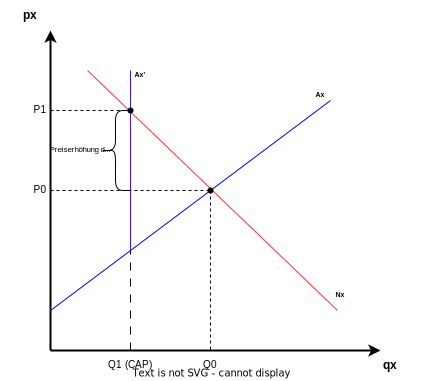
\includegraphics[width=0.8\textwidth]{Bilder/supply_demand_ets.png} 
	\caption{Angebot und Nachfrage von Emissionszertifikaten mit CAP (vgl. \cite{pettinger.2017})}
	\label{fig:supply_demand_ets}
\end{figure}
\chapter{Praxis}

Aktuell sind in Deutschland zwei Emissionshandelssysteme aktiv. Zum einen das EU-Emissionshandelssystem (ETS) geregelt durch das 'EU ETS legislative framework' \cite{eu.2023} und zum anderen das deutsche nationale Emissionshandelssystem (nEHS), das durch das 'Brennstoffemissionshandelsgesetz' (BEHG) geregelt wird \cite{dehst.2023}.

\section{EU-Emissionshandelssystem (ETS)}

Das ETS ist das weltweit größte Emissionshandelssystem. Es wurde 2005 eingeführt und deckt ca. 40\% der Treibhausgasemissionen der EU ab. Das ETS gilt für den europäischen Binnenmarkt sowie für die Staaten Island, Lichtenstein und Norwegen. Es zielt auf direkte Emissionen aus der produzierenden Industrie, dem Energiesektor und der Luftfahrt ab. Ab 2024 sind auch Emissionen aus der Schiffahrt vom ETS gedeckt \cite{eu.2023}.
Bei dem ETS handelt es sich um einen s.g. Downstream Emissionshandel \cite{dehst.2023}. Das bedeutet, dass Emittenten die Berechtigung für ihre Emissionen selbst erwerben. Das bedeutet, dass die Emittenten von sich aus den Anreiz haben, ihre CO2e-Austoß zu senken.  

\chapter{Fazit}

Emissionshandelssysteme sind als marktwirtschaftliches Instrument gegen den Klimawandel einzigartig aufgrund ihrer ökologischen Treffsicherheit (vgl. \cite[S. 182]{hubert.2020}).
Dies ist auf den sinkenden Emissions-Cap einer Volkswirtschaft zurückzuführen, mit dem die Menge der ausgestoßenen Treibhausgase kontrolliert werden kann.
Voraussetzung dafür ist, dass der Cap nicht zu hoch angesetzt wird, wie am Negativbeispiel der Zertifikatsmenge des EU ETS nach der Finanzkrise gesehen werden kann (vgl. \cite{eu3.2023}).

Ein weiterer Vorteil ist die ökonomische Effizienz. Unternehmen und Verbraucher haben selbst die Wahl, wie sie ihre Emissionen reduzieren.
Sie können selbst entscheiden, wo sie Emissionen vermeiden wollen und wo nicht. Langfristig kann kein Verbraucher das Problem des Treibhausgasausstoßes ignorieren, da sonst die Kosten für seine Emissionen zu hoch werden.
So gibt es Anreize für den privaten Sektor, Geld in die Forschung und Entwicklung klimafreundlicherer Technologien zu investieren (vgl. \cite[S. 183]{hubert.2020}).
Dennoch besteht das Problem, dass es keinen weltweit einheitlichen $CO_2$-Preis gibt und so Hersteller, die in Volkswirtschaften produzieren, die keinen oder nur einen geringen $CO_2$-Preis haben, einen Wettbewerbsvorteil erlangen können.
Das Beispiel des EU ETS hat jedoch gezeigt, dass importierte Treibhausgase nachträglich über Werkzeuge wie den 'Carbon Border Adjustment Mechanism' (CBAM) erfasst werden können und so der $CO_2$-Preis nachträglich auf alle importierten Güter angewendet werden kann (vgl. \cite{ub.2023}).

Bei der Praktikabilität stellt sich die Frage, wie die Zertifikate am besten ausgegeben werden sollen. Der EU ETS hat gezeigt, dass sich ein Downstream-System besonders für große Verursacher in der Industrie eignet.
Die Verteilung durch Auktionen hat sich hier besonders bewährt. Um kleinere Verursacher zu erreichen, können Upstream-Systeme wie das nEHS eingesetzt werden, indem die Verursacher indirekt für ihre Emissionen zahlen müssen.

Alles in allem ist ein Emissionshandelssystem ein gutes Instrument, um marktwirtschaftliche Volkswirtschaften zur Klimaneutralität zu bewegen.
\chapter{Materialanhang}

\begin{figure}[ht]
	\centering
	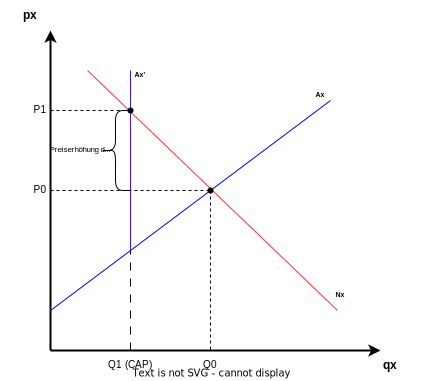
\includegraphics[width=0.8\textwidth]{Bilder/supply_demand_ets.png} 
	\caption{Angebot und Nachfrage von Emissionszertifikaten mit CAP (vgl. \cite{pettinger.2017})}
	\label{fig:supply_demand_ets}
\end{figure}

\begin{figure}[ht]
	\centering
	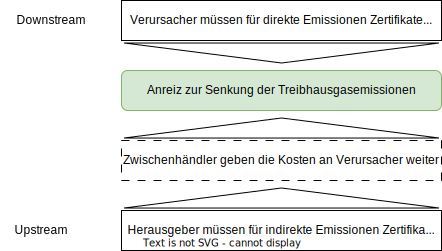
\includegraphics[width=0.8\textwidth]{Bilder/up_and_downstream_ets.png} 
	\caption{Anreize für Verursacher über Upstream- und Downstream-Systeme (vgl. \cite{dehst.2023})}
	\label{fig:up_and_downstream_ets}
\end{figure}

\begin{figure}[ht]
	\centering
	\includegraphics[width=1.0\textwidth]{Bilder/price_co2_eu_ets.png} 
	\caption{Preisentwicklung in € für Emissionsberechtigungen im EU ETS seit 2008 als $CO_2$e-Preis pro Tonne (\cite{dehst.2023})}
	\label{fig:price_co2_eu_ets}
\end{figure}

\begin{figure}[ht]
	\centering
	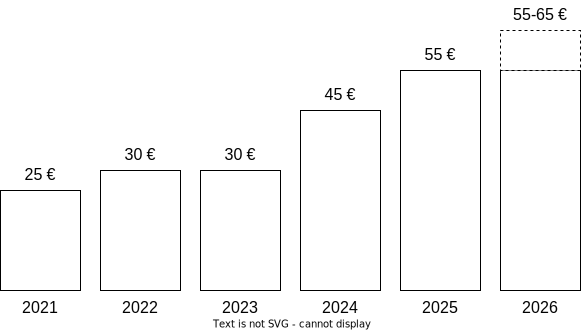
\includegraphics[width=1.0\textwidth]{Bilder/prices_nehs.png} 
	\caption{Preisentwicklung $CO_2$e-Preis pro Tonne für den nEHS (\cite{dehst.2023})}
	\label{fig:prices_nehs}
\end{figure}

% ---- Literaturverzeichnis
\cleardoublepage
\renewcommand*{\chapterpagestyle}{plain}
\pagestyle{plain}
\pagenumbering{Roman}                   % Römische Seitenzahlen
\setcounter{page}{\numexpr\value{savepage}+1}
\printbibliography[title=Literaturverzeichnis]

% ---- Anhang
\appendix
%\clearpage
%\pagenumbering{Roman}  % römische Seitenzahlen für Anhang

\newpage
\end{document}